\documentclass[11pt,a4paper]{article}

\usepackage[spanish]{babel}
\usepackage[utf8]{inputenc}
\usepackage{amsmath, amssymb}
\usepackage{graphicx}
\usepackage{float}
\usepackage{geometry}
\usepackage{booktabs}
\usepackage{physics}
\usepackage{siunitx}
\usepackage{subcaption}
\usepackage{multirow}
\usepackage{listings}
\decimalpoint

\geometry{margin=2.5cm}

\title{Paseos aleatorios y difusión en 2D}
\author{Andrés López Serna}
\date{\today}

\begin{document}

\maketitle

\begin{abstract}

En este trabajo se estudia la equivalencia entre los paseos aleatorios y la ecuación de difusión en dos dimensiones mediante simulaciones numéricas. Se demuestra que tanto el paseo aleatorio presenta un crecimiento lineal del desplazamiento cuadrático medio. Posteriormente se integra numéricamente la ecuación de difusión y se obtiene el mismo comportamiento. Finalmente, se analiza la evolución de la entropía del sistema bajo condiciones periódicas de frontera, observando su acercamiento al límite hacia el equilibrio. Como extensión, se incluye un estudio de las curvas de Koch como ejemplo de estructura fractal.

\end{abstract}

\section{Introducción}

Los procesos de difusión aparecen en múltiples sistemas físicos y pueden describirse tanto desde un punto de vista microscópico como macroscópico.

El paseo aleatorio constituye un modelo fundamental para describir el movimiento de partículas de forma discreta, mientras que la ecuación de difusión proporciona una descripción continua de la evolución de la densidad.

El objetivo de esta práctica es esclarecer la conexción entre ambos enfoques mediante simulaciones numéricas. Finalmente, se analizará la evolución de la entropía del sistema y, adicionalmente, se estudiará el caso de una objeto de dimensión fractal: las curvas de Koch.

\section{Marco teórico}

\subsection{Paseo aleatorio}

En dos dimensiones, cada caminante realiza en cada paso temporal dos desplazamientos independientes de distancias $d_x= d_y = 1$.

\begin{equation}
x_{n+1} = x_n \pm d_x, \quad y_{n+1} = y_n \pm d_y
\end{equation}

Estos desplazamientos cumplen que el valor esperado de la posición al cuadrado tras n pasos coincide con el número de pasos:

\begin{equation}
\langle x^2 \rangle =\langle \sum^n_is_i\sum^n_js_j \rangle =\langle \sum^n_i\sum^n_j(s_is_j) \rangle =\langle \sum^n_is_i^2 \rangle =\langle \sum^n_i1 \rangle = n
\end{equation}

Teniendo en cuenta que $r^2=x^2+y^2$, y que las coordenadas x e y se pueden tratar de forma independiente, en 2D, se cumple lo siguiente:

\begin{equation}
\langle r^2 \rangle =\langle x^2+y^2 \rangle =\langle x^2 \rangle +\langle y^2 \rangle = 2n
\end{equation}
 
\subsection{Ecuación de difusión}

La ecuación de difusión en 2D utilizando la distribución de probabilidad es:

\begin{equation}
\frac{\partial \rho}{\partial t} = D \left( \frac{\partial^2 \rho}{\partial x^2} + \frac{\partial^2 \rho}{\partial y^2} \right)
\end{equation}

Las soluciones de esta ecuación tienen forma de gaussiana, en 2D es:

\begin{equation}
\rho(x,y,t)=\frac{1}{4\pi Dt}exp(-\frac{x^2+y^2}{4Dt})
\end{equation}

A partir de esta solución se puede obtener el valor esperado de la posición en 2D llegando a la siguiente relación:

\begin{equation}
\langle r^2 \rangle = \int r^2 \frac{1}{4\pi Dt}exp(-\frac{r^2}{4Dt})d\vec{r}=4Dt
\end{equation}

Por tanto, tanto los caminantes aleatorios como las soluciones de la ecuación de difusión mantienen una tendencia lineal y su pendiente es igual si $D=\frac{1}{2}$.

\subsection{Entropía}

Para cuantificar el grado de desorden del sistema se utiliza la entropía de Shannon, asociada a la distribución de probabilidad discreta:

\begin{equation}
S(t) = -\sum_i P_i(t)\,\ln P_i(t)
\end{equation}

donde $P_i(t)$ es la probabilidad de encontrar una partícula en la celda $i$ en el instante $t$.

Esta magnitud permite caracterizar la evolución del sistema desde estados más ordenados (baja entropía) hacia estados más desordenados (alta entropía). En particular, si todas las partículas están concentradas en una región pequeña del espacio, la distribución es altamente no uniforme y la entropía es baja, mientras que si las partículas están distribuidas homogéneamente, la entropía alcanza su valor máximo.

En el caso de una malla discreta de $M$ celdas, la entropía máxima se alcanza cuando todas las probabilidades son iguales ($P_i = \frac{1}{M}$) lo que conduce a:

\begin{equation}
S_{\text{max}} = \ln M
\end{equation}

En el caso de esta práctica, al discretizar el espacio en una malla de $10 \times 10$ celdas, se tiene $M = 100$, por lo que $S_{\text{max}} = \ln(100)$.

Bajo condiciones de contorno periódicas, el sistema evoluciona hacia un estado estacionario homogéneo, por lo que se espera que la entropía crezca con el tiempo hasta saturarse en este valor máximo.

\section{Métodos numéricos}

\subsection{Distribución inicial}

Para evitar utilizar pasos temporales bajos y evitar que los resultados del caminante aleatorio sean todos de la misma paridad. [\ref{Giordano}] Se ha utilizado una condición inicial distribuida uniformemente en el cuadrado $[-5,5]\times[-5,5]$, tanto para el estudio de la difusión como para los caminantes aleatorio.

\subsection{Condición de estabilidad}

Para determinar el paso temporal, se emplea un esquema el caso límite (la igualdad) que cumple la condición de estabilidad para el tratamiento numérico de diferencias finitas (condición de Courant):

\begin{equation}
\Delta t \le \frac{1}{2D\left(\frac{1}{dx^2} + \frac{1}{dy^2}\right)}
\end{equation}

\subsection{Condiciones de contorno periódicas}

Se imponen condiciones de contorno periódicas mediante:

\begin{equation}
x = x + L 
\end{equation}
\begin{equation}
y = y + L 
\end{equation}

lo que hace que las partículas que abandonan la caja de dimensiones $L \times L$ reaparezcan por el lado opuesto.

\section{Resultados}

\subsection{Paseo aleatorio y difusión}

Coincidiendo con lo pronosticado en el apartado teórico, se obtiene un crecimiento lineal de $\langle r^2 \rangle$, tanto para los caminantes aleatorios como para la difusión. Además, la pendiente obtenida ajustando los datos a una recta coincide con lo esperado.

\begin{table}[H]
\centering
\begin{tabular}{|c|c|c|}
\hline
Modelo & Pendiente (ajuste) & Valor teórico \\
\hline
Paseo aleatorio 2D & $1.97$ & $2$ \\
\hline
Difusión 2D & $2.00$ & $4D = 2$ \\
\hline
\end{tabular}
\caption{Comparación entre las pendientes obtenidas mediante ajuste lineal del desplazamiento cuadrático medio y los valores teóricos esperados.}
\label{tab:msd}
\end{table}

\begin{figure}[H]
\centering
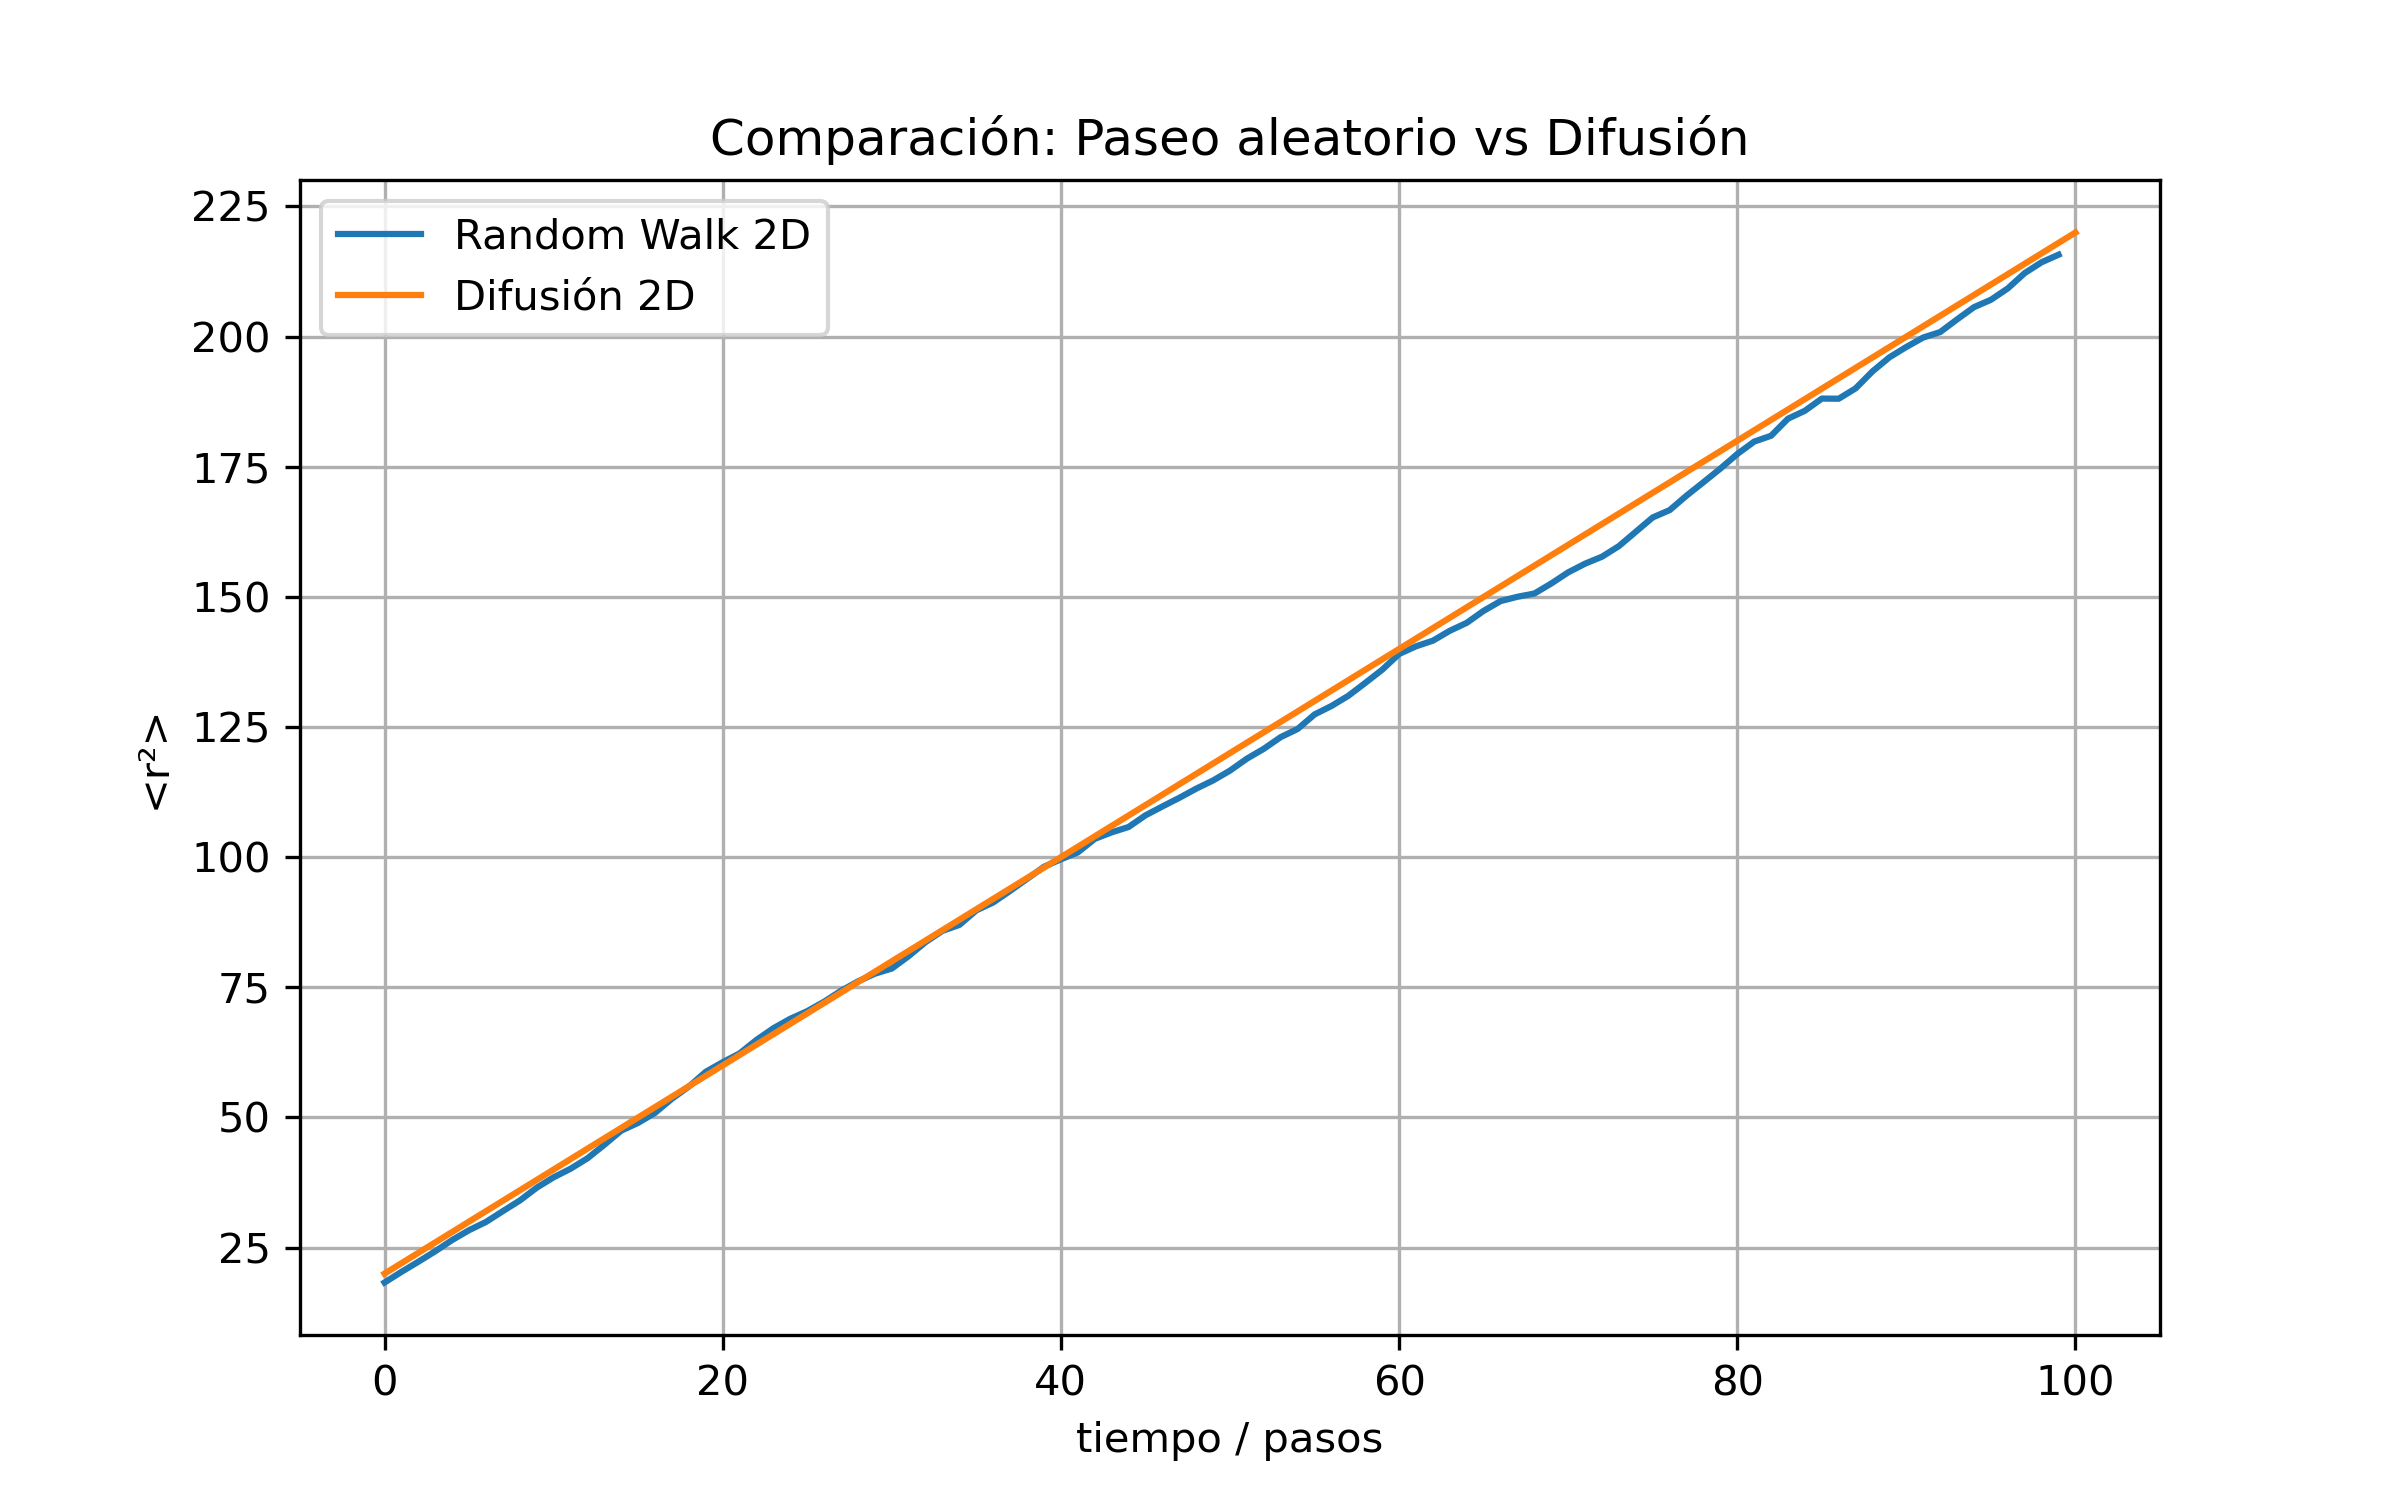
\includegraphics[width=0.6\textwidth]{imagenes/rw_vs_dif.png}
\caption{Comparación entre paseo aleatorio y difusión.}
\end{figure}

De la gráfica comparativa de los caminantes aleatorios y la difusión, caben destacar, además de los valores de pendiente, que su ordenada en el origen es la misma para ambos casos.

\subsection{Evolución de la difusión}

\begin{figure}[H]
\centering
\begin{subfigure}{0.32\textwidth}
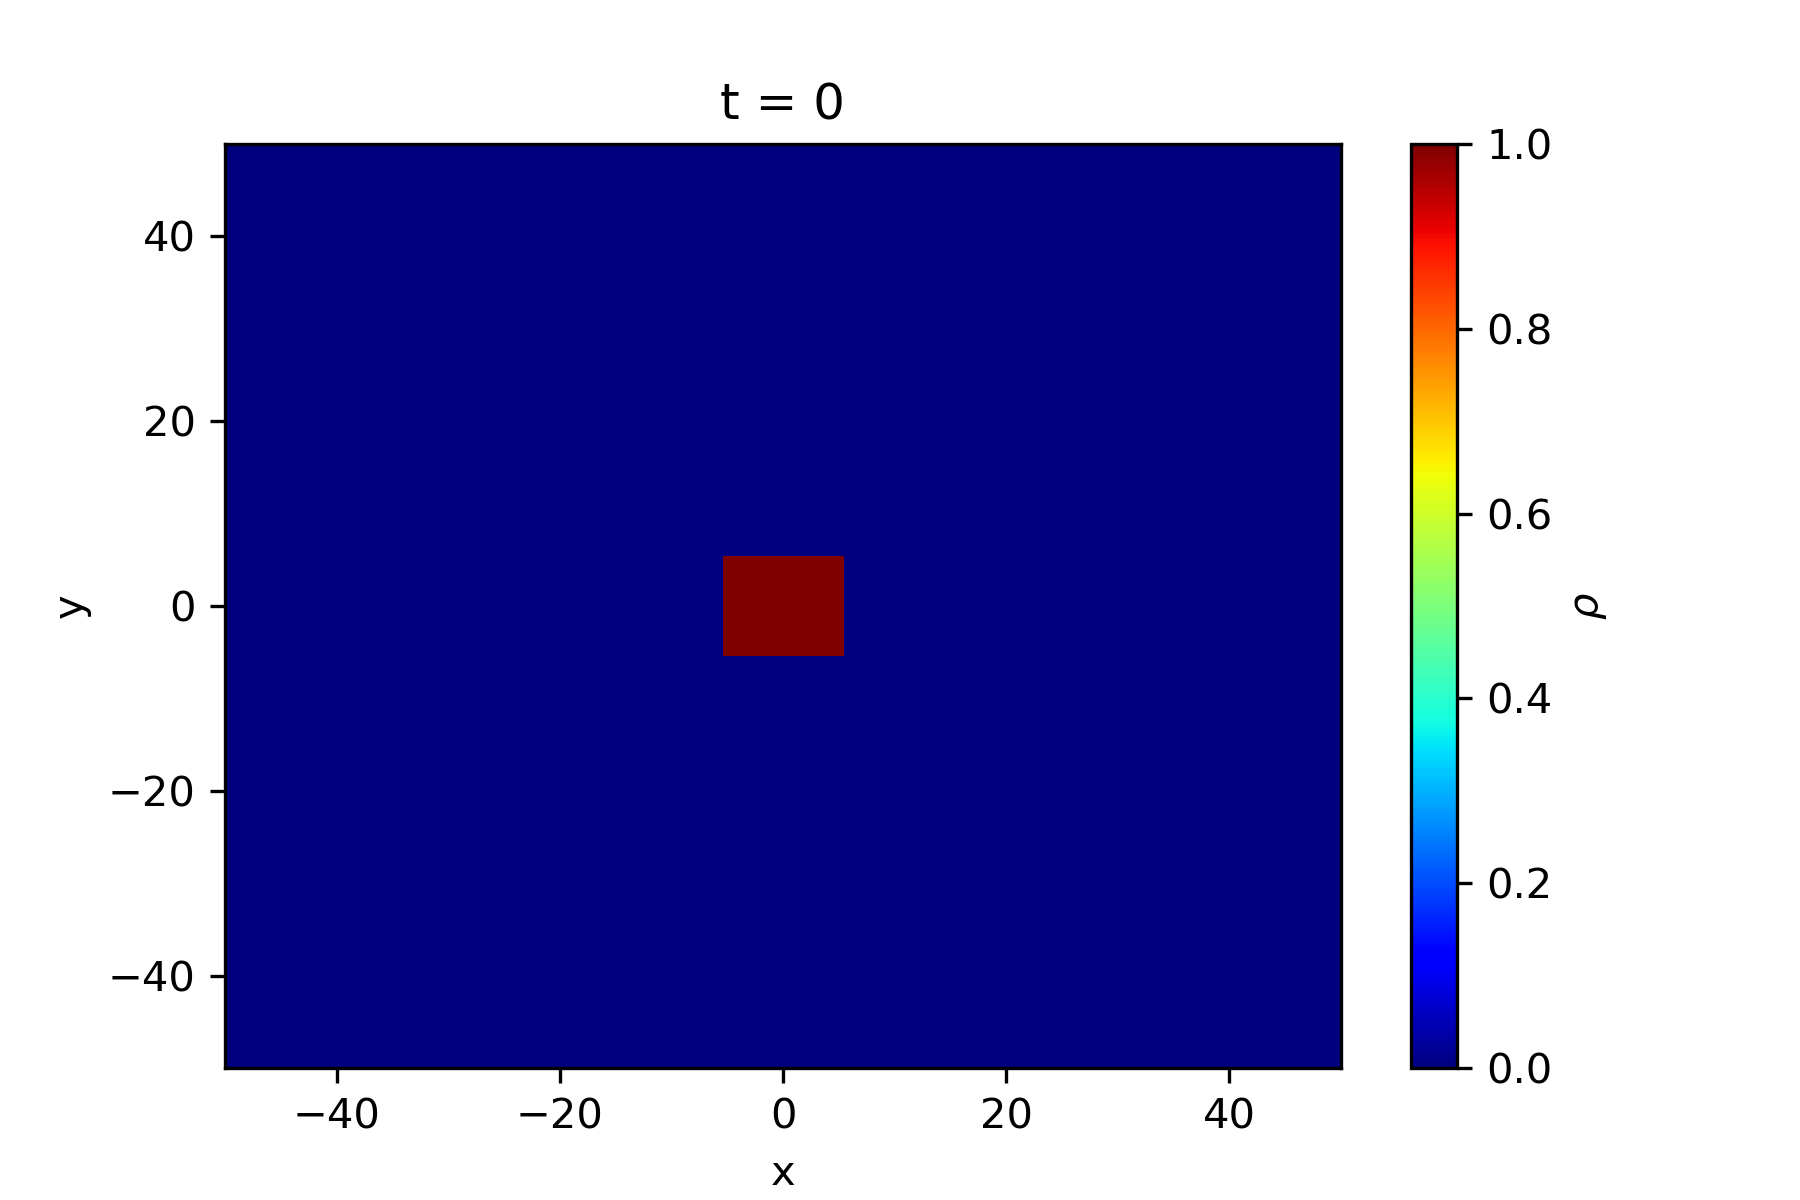
\includegraphics[width=\linewidth]{imagenes/t=0.png}
\caption{$t=0$}
\end{subfigure}
\begin{subfigure}{0.32\textwidth}
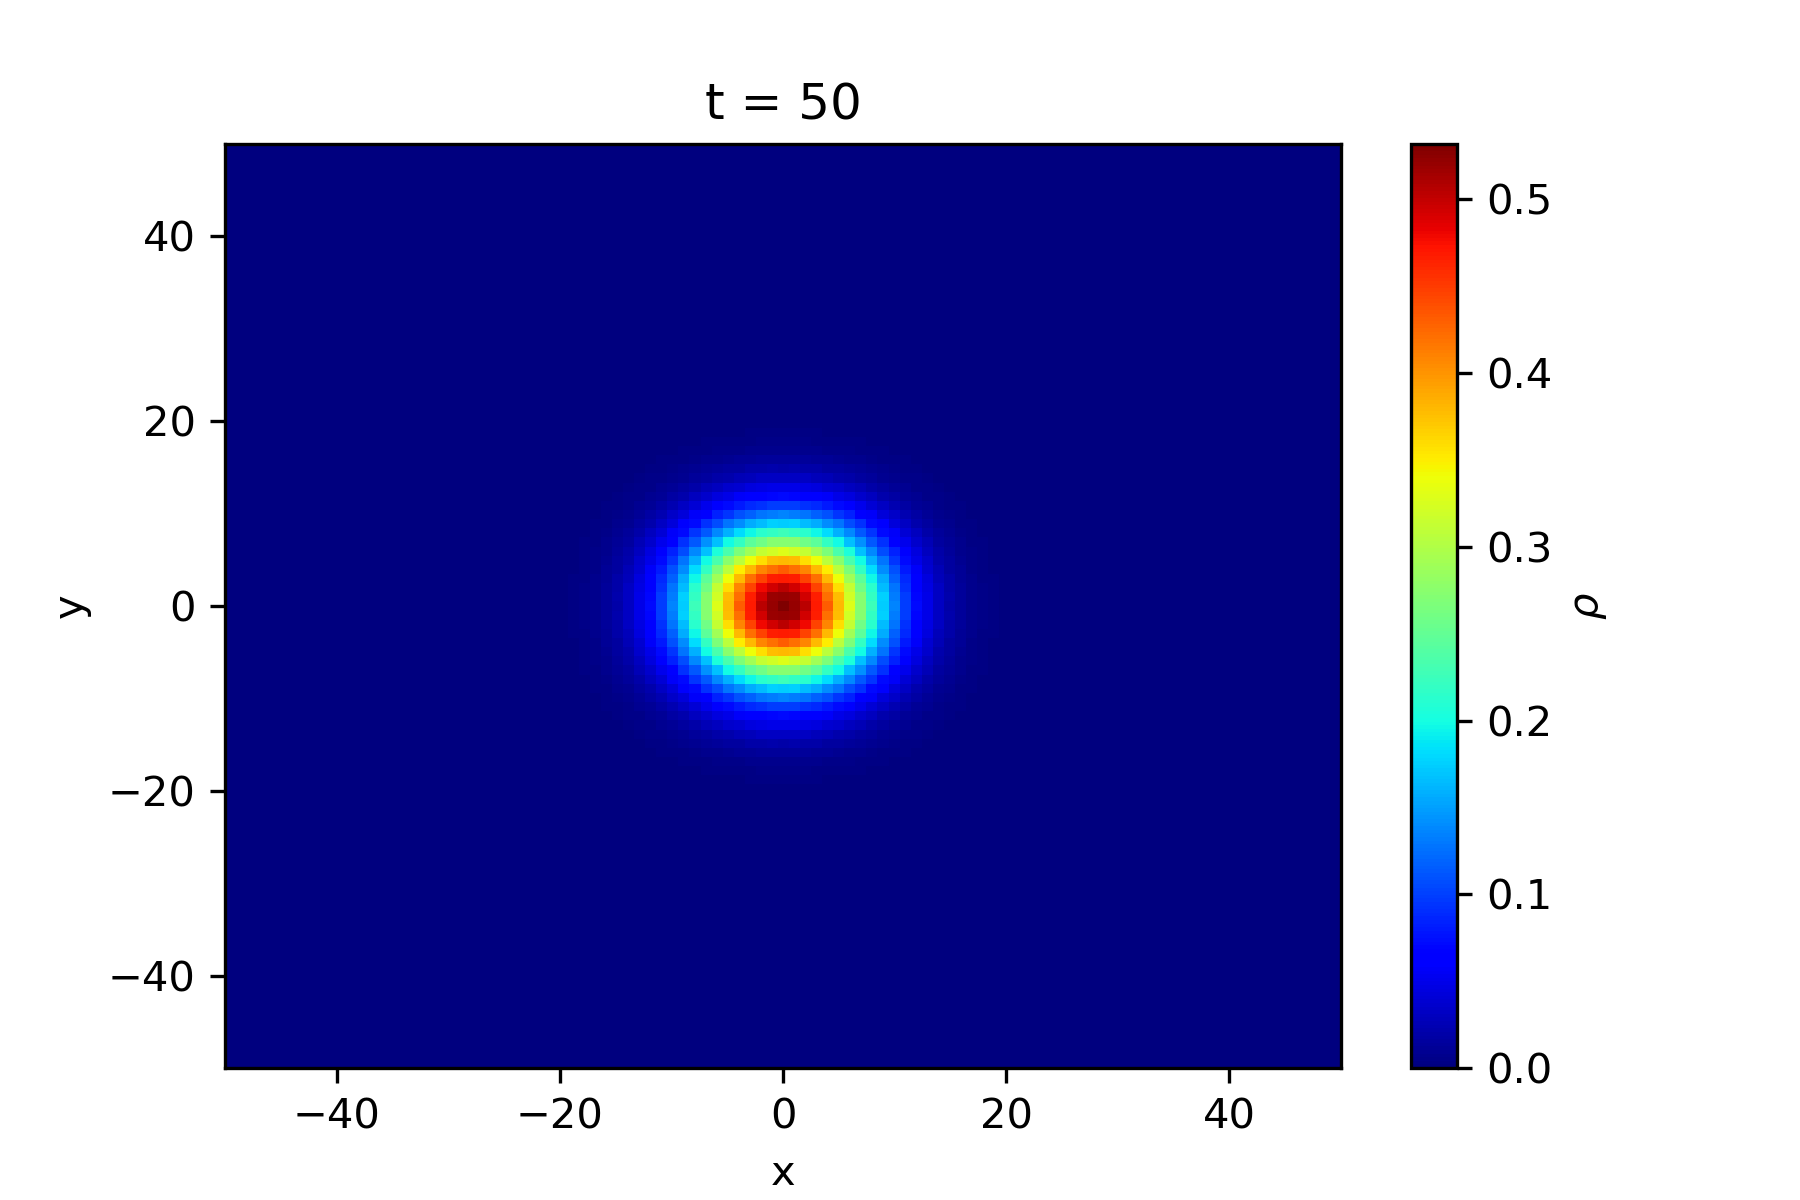
\includegraphics[width=\linewidth]{imagenes/t=50.png}
\caption{$t=50$}
\end{subfigure}
\begin{subfigure}{0.32\textwidth}
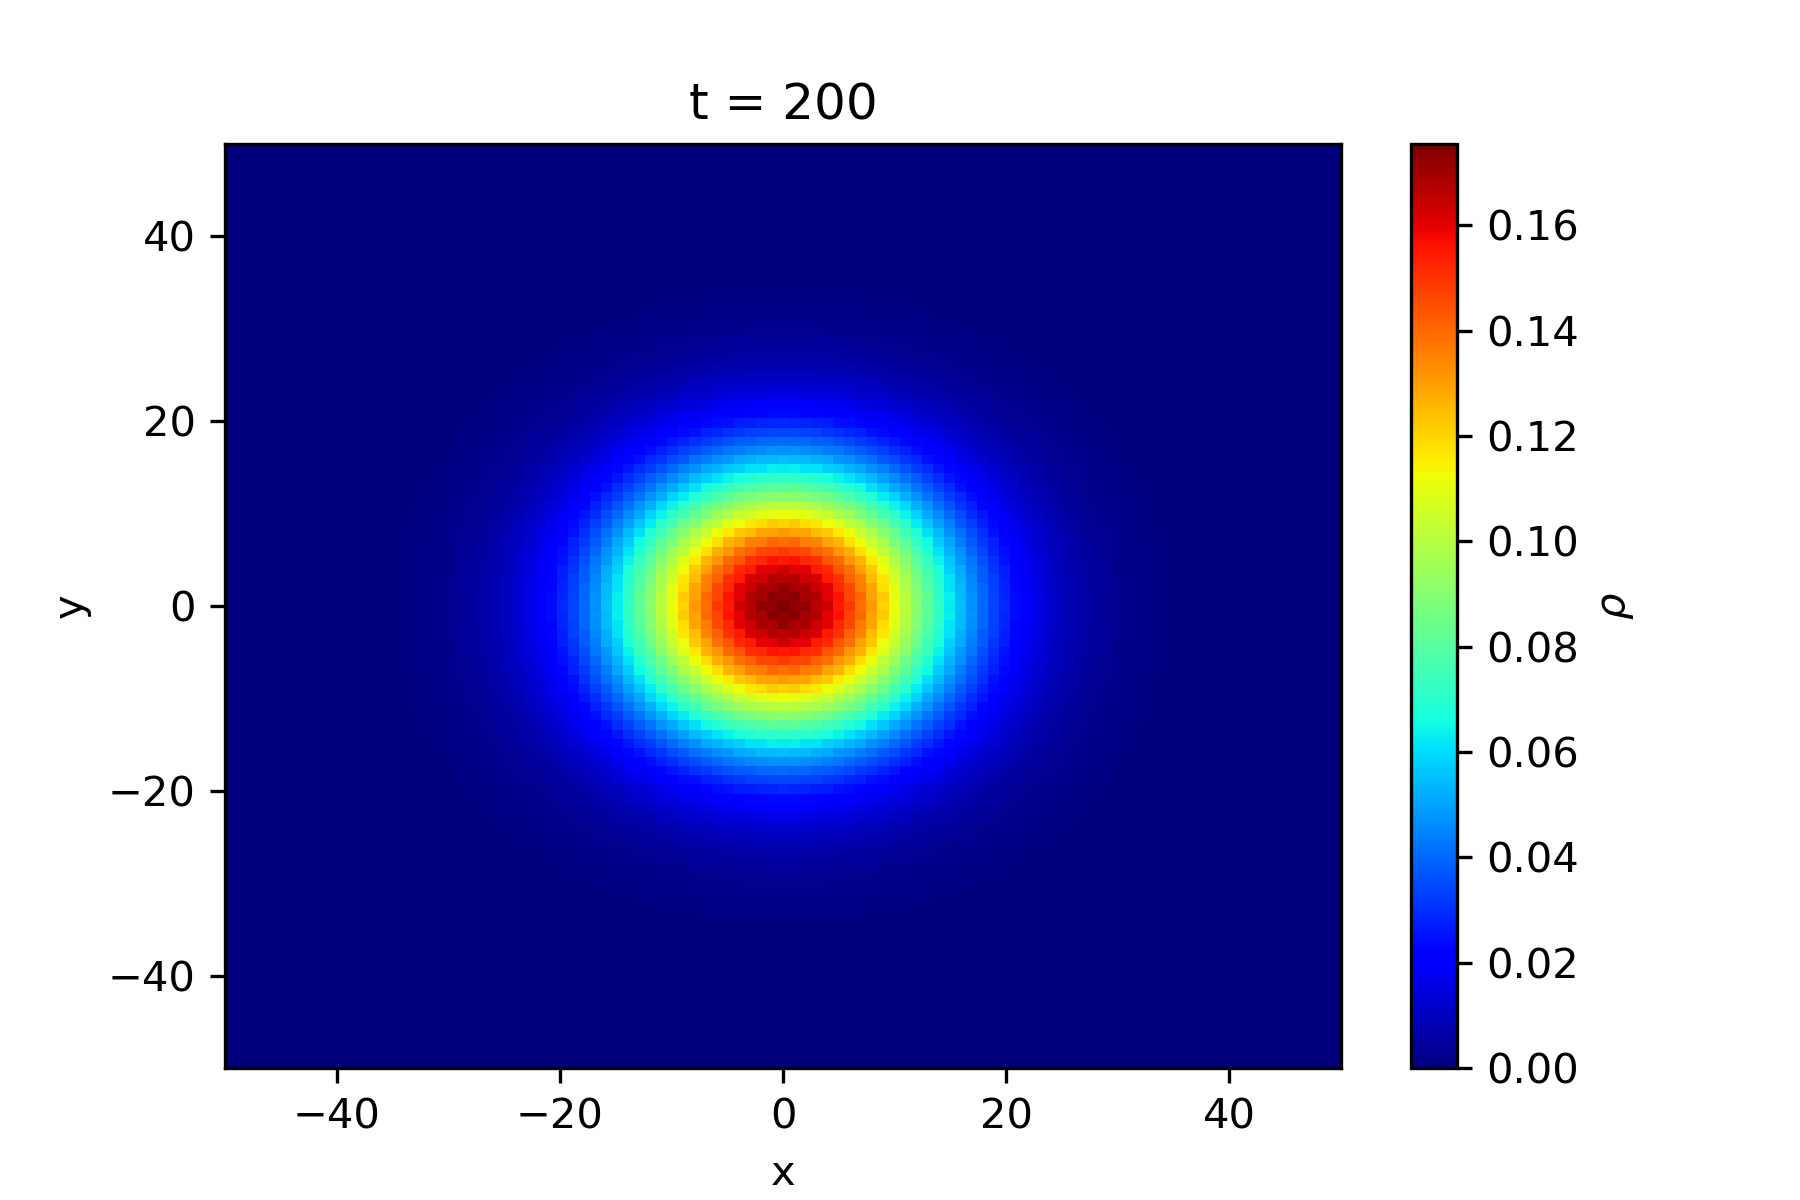
\includegraphics[width=\linewidth]{imagenes/t=200.png}
\caption{$t=200$}
\end{subfigure}
\caption{Evolución de la densidad de probabilidad.}
\end{figure}

Se observa la expansión progresiva de la distribución de probabilidad, que, cuando t aumenta se homogeneiza hasta llegar a una distribución totalmente homogénea.

\subsection{Entropía}

\begin{figure}[H]
\centering
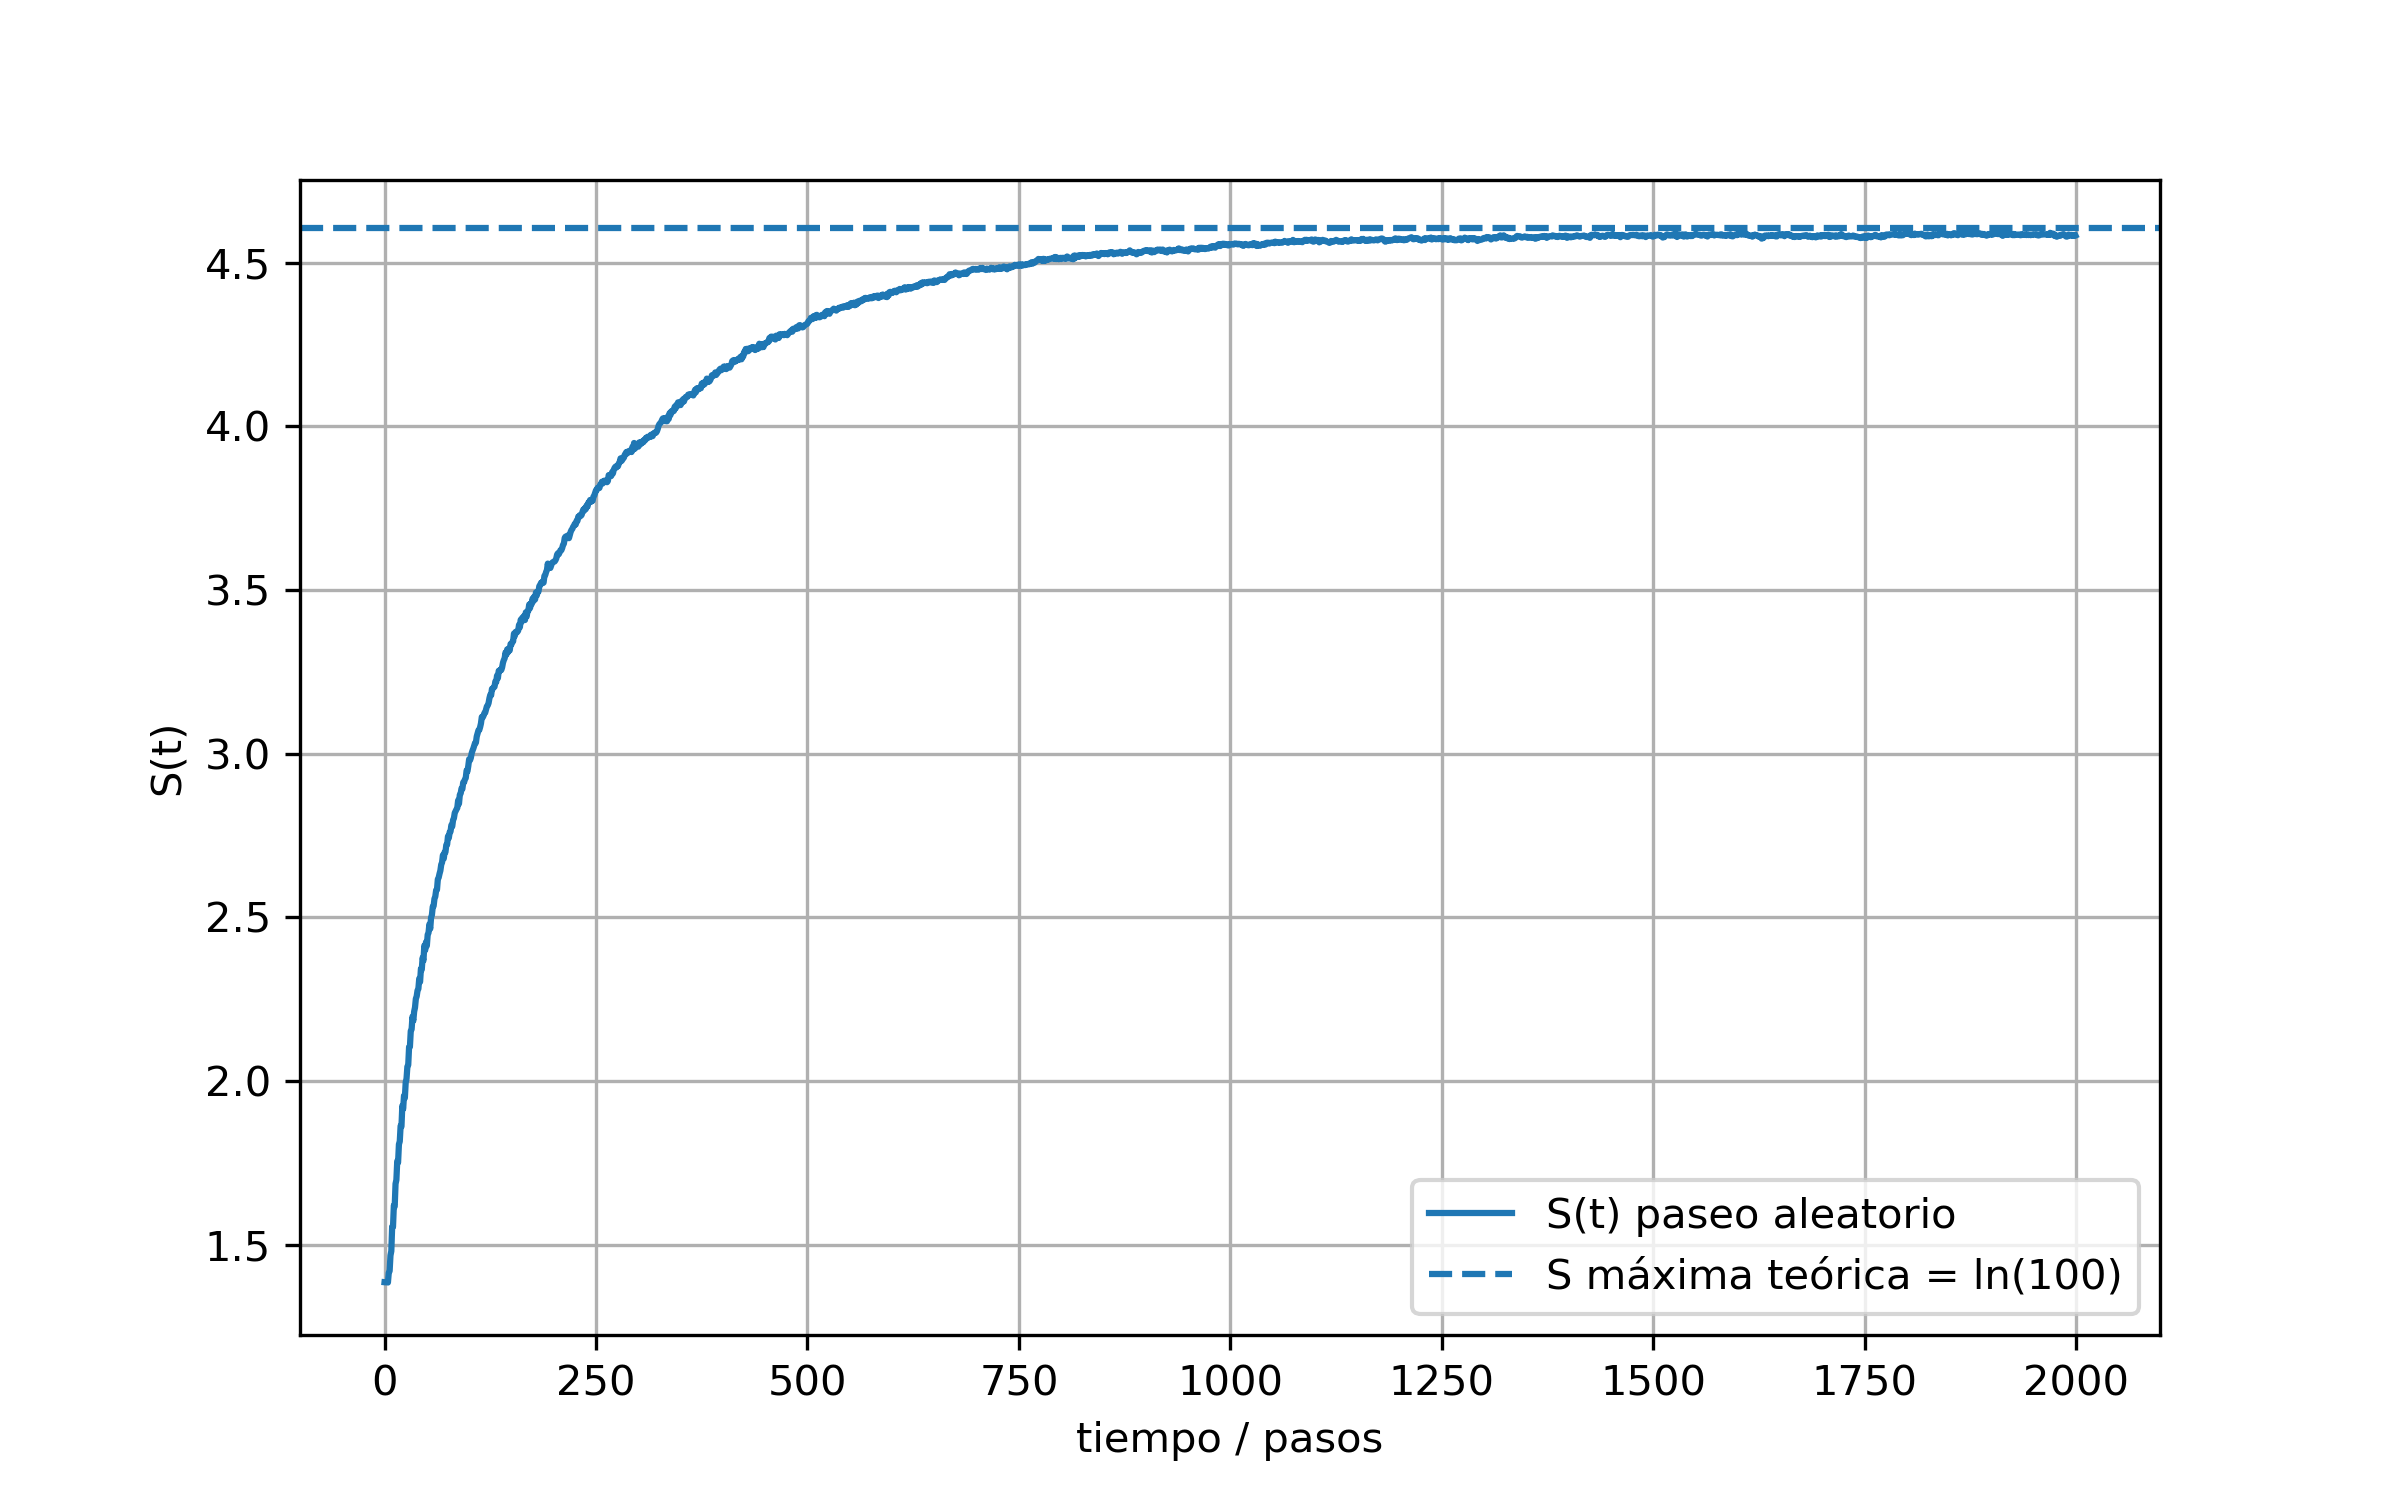
\includegraphics[width=0.6\textwidth]{imagenes/evolucion_entropia.png}
\caption{Evolución temporal de la entropía.}
\end{figure}

Como se podría esperar, debido a la dispersión de los caminantes aleatorios, la entropía crece inicialmente, desde un estado de baja entropía (distribución inicial ordenada) hasta acercarse al límite teórico, donde el resultado se estabiliza ya que todas las partículas se encuentran en el estado de máxima mezcla (distribución homogénea). Esto refleja la llegada al equilibrio bajo condiciones periódicas.

\subsection{Extensión: Curva de Koch}

Como extensión del trabajo, se han implementado la curvas de Koch como ejemplos de estructuras fractales.

\begin{figure}[H]
\centering

\begin{subfigure}{0.3\textwidth}
\centering
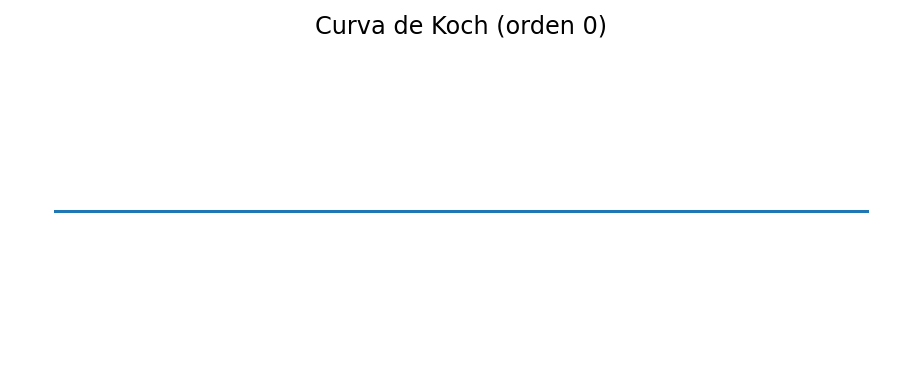
\includegraphics[width=\linewidth]{imagenes/orden0.png}
\caption{$n=0$}
\end{subfigure}
\hfill
\begin{subfigure}{0.3\textwidth}
\centering
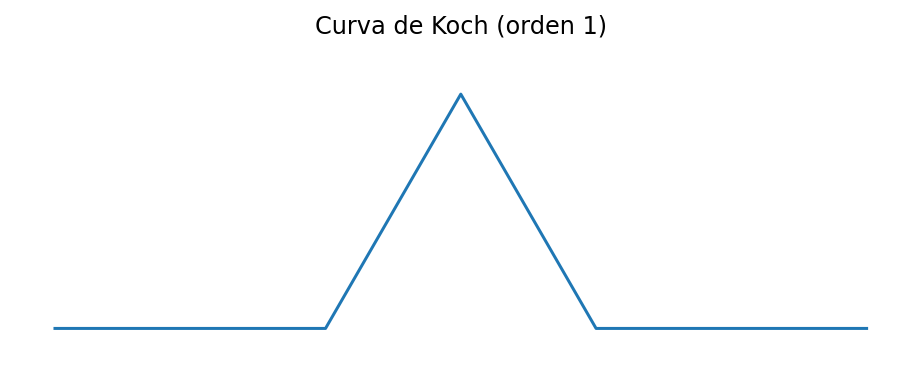
\includegraphics[width=\linewidth]{imagenes/orden1.png}
\caption{$n=1$}
\end{subfigure}
\hfill
\begin{subfigure}{0.3\textwidth}
\centering
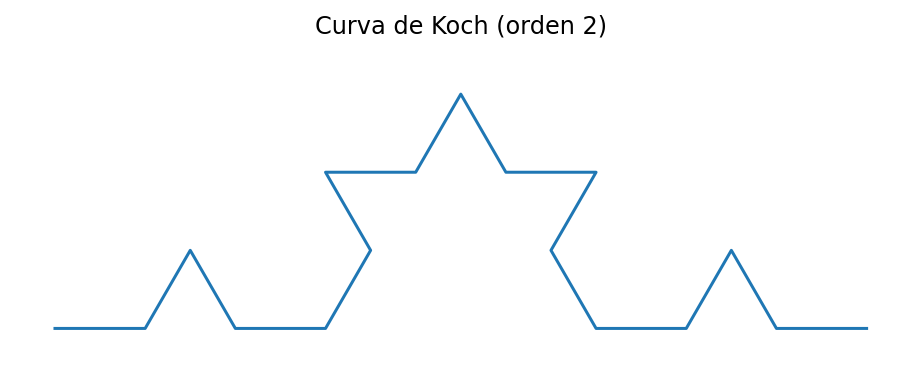
\includegraphics[width=\linewidth]{imagenes/orden2.png}
\caption{$n=2$}
\end{subfigure}

\vspace{0.3cm}

\begin{subfigure}{0.3\textwidth}
\centering
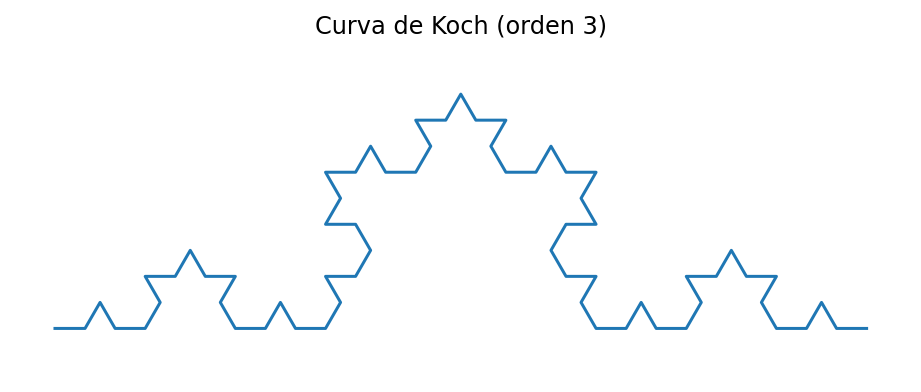
\includegraphics[width=\linewidth]{imagenes/orden3.png}
\caption{$n=3$}
\end{subfigure}
\hfill
\begin{subfigure}{0.3\textwidth}
\centering
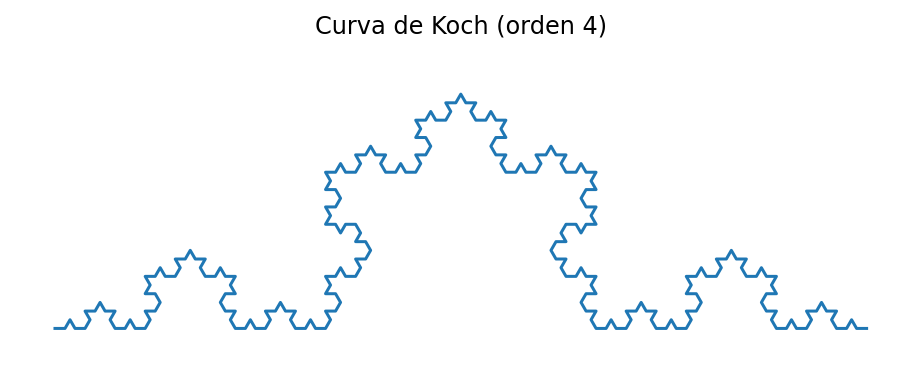
\includegraphics[width=\linewidth]{imagenes/orden4.png}
\caption{$n=4$}
\end{subfigure}
\hfill
\begin{subfigure}{0.3\textwidth}
\centering
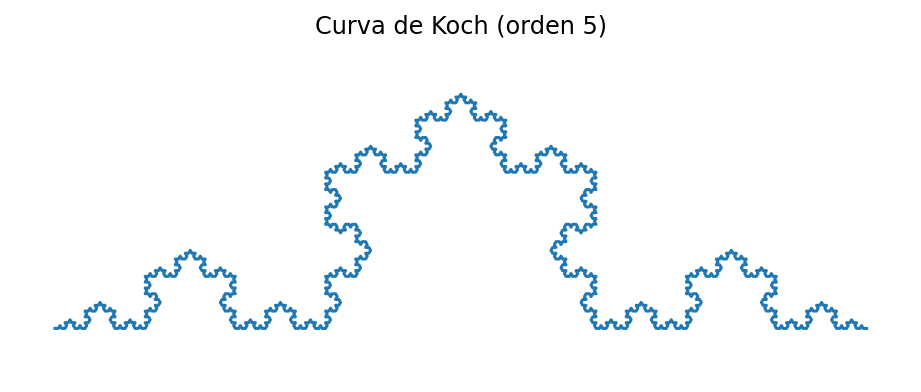
\includegraphics[width=\linewidth]{imagenes/orden5.png}
\caption{$n=5$}
\end{subfigure}

\caption{Evolución de la curva de Koch para distintos órdenes.}
\label{fig:koch}
\end{figure}y

\subsubsection{Construcción de la curva}

La curva de Koch se construye de manera recursiva a partir de un segmento inicial. En cada iteración, cada segmento se divide en tres partes iguales y se sustituye el segmento central por dos segmentos que formarían un triángulo equilátero con dicho segmento.

Este procedimiento genera, en cada iteración, una curva cada vez más irregular, aumentando el número de segmentos según $N_n = 4^n$ y reduciendo la longitud de cada segmento en un factor $1/3$.

\subsubsection{Longitud de la curva}

La longitud total de la curva en la iteración $n$ viene dada por

\begin{equation}
L_n = \left(\frac{4}{3}\right)^n
\end{equation}

lo que implica que la longitud crece exponencialmente con el número de iteraciones.

Numéricamente, se ha calculado la longitud sumando las distancias entre puntos consecutivos. Los resultados obtenidos coinciden con la expresión teórica, presentando errores muy pequeños debidos a la discretización numérica. Se observa claramente el crecimiento divergente de la longitud, característico de estructuras fractales.

\begin{figure}[H]
\centering
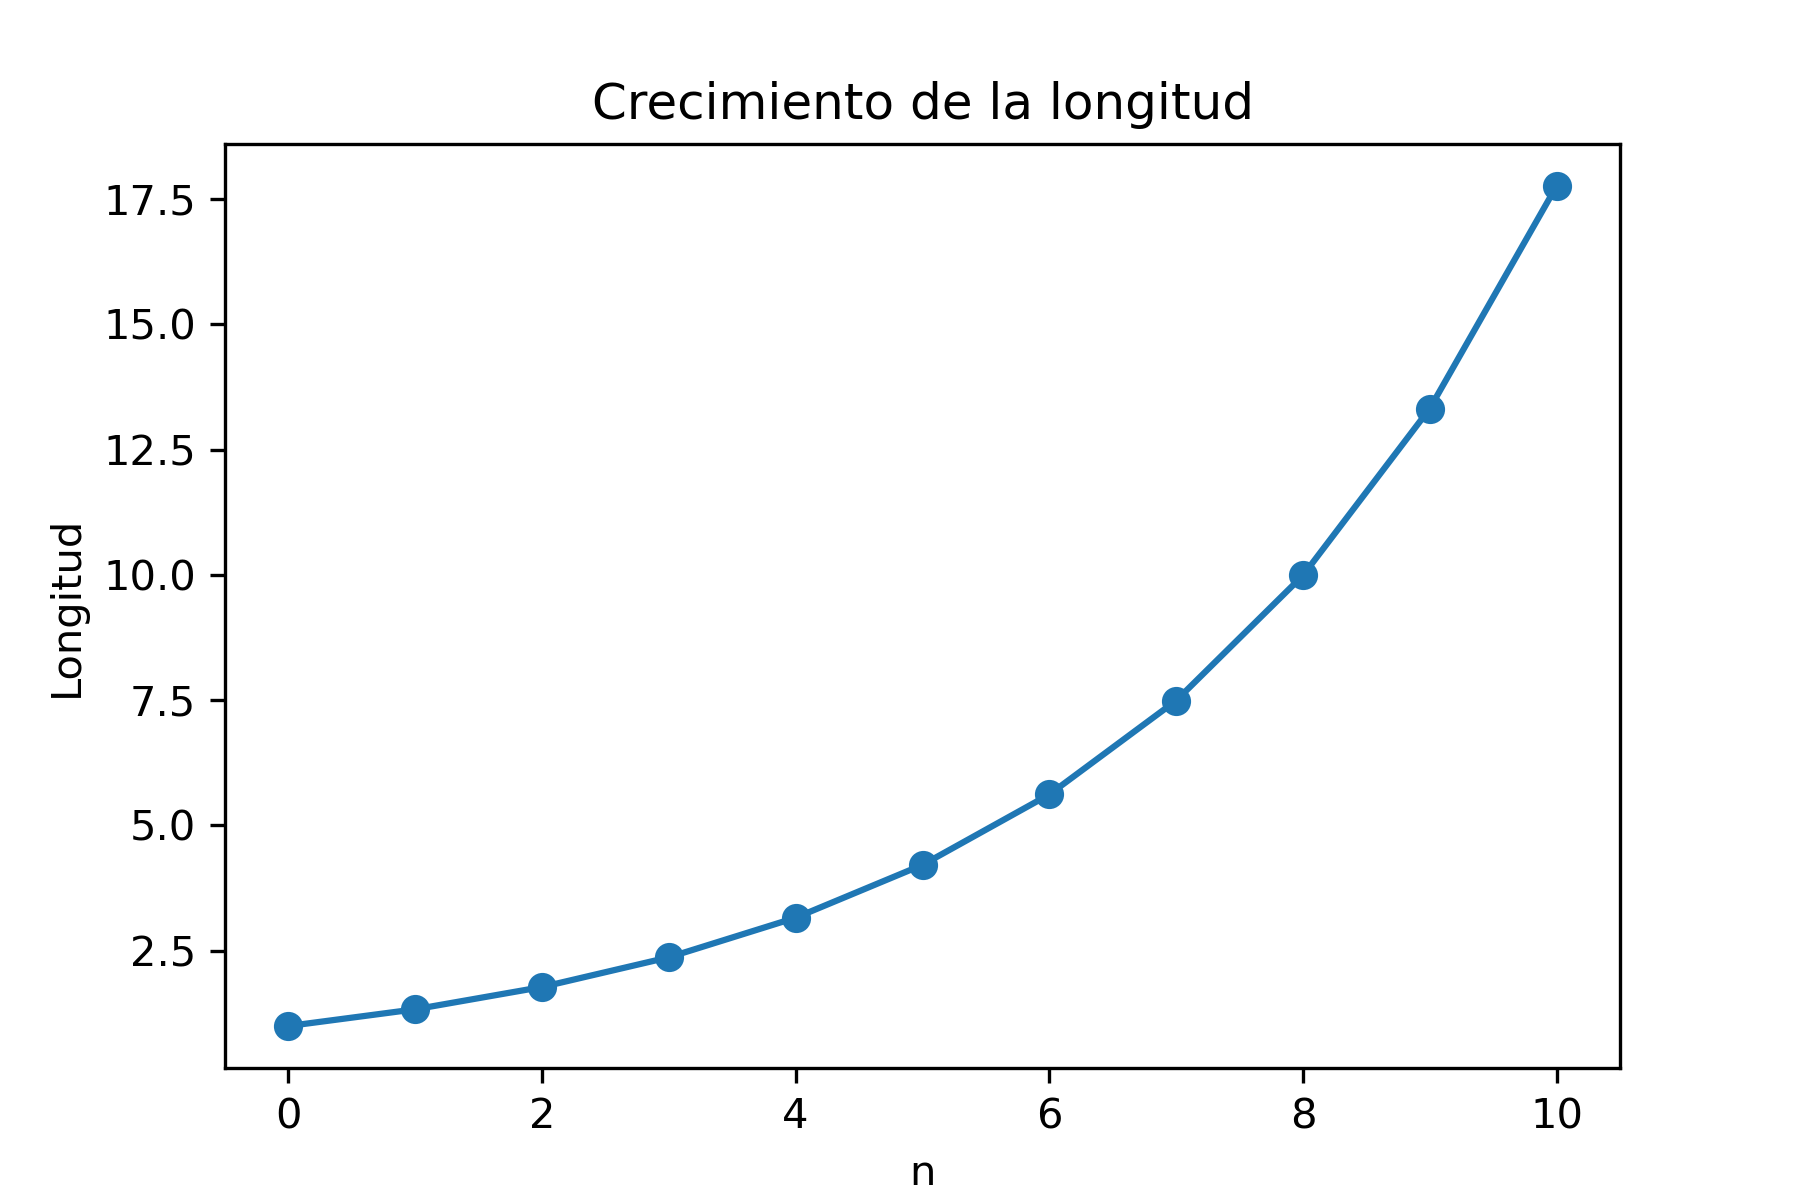
\includegraphics[width=0.6\textwidth]{imagenes/long_koch.png}
\caption{Evolución de la longitud de la curva de Koch al aumentar el número de iteraciones.}
\end{figure}


\subsubsection{Área del copo de Koch}

A pesar de que la longitud diverge, el área encerrada por el copo de Koch (área contenida entre la curva de Koch de orden n y la curva de orden 0) converge a un valor finito. El área se obtiene sumando las contribuciones de los triángulos añadidos en cada iteración:

\begin{equation}
A_n = A_0 + \sum_{k=1}^{n} 3 \cdot 4^{k-1} \cdot \frac{A_0}{9^k}
\end{equation}

donde $A_0$ es el área del triángulo inicial.

En el límite $n \to \infty$, el área converge a

\begin{equation}
A_{\infty} = \frac{8}{5} A_0
\end{equation}

\begin{figure}[H]
\centering
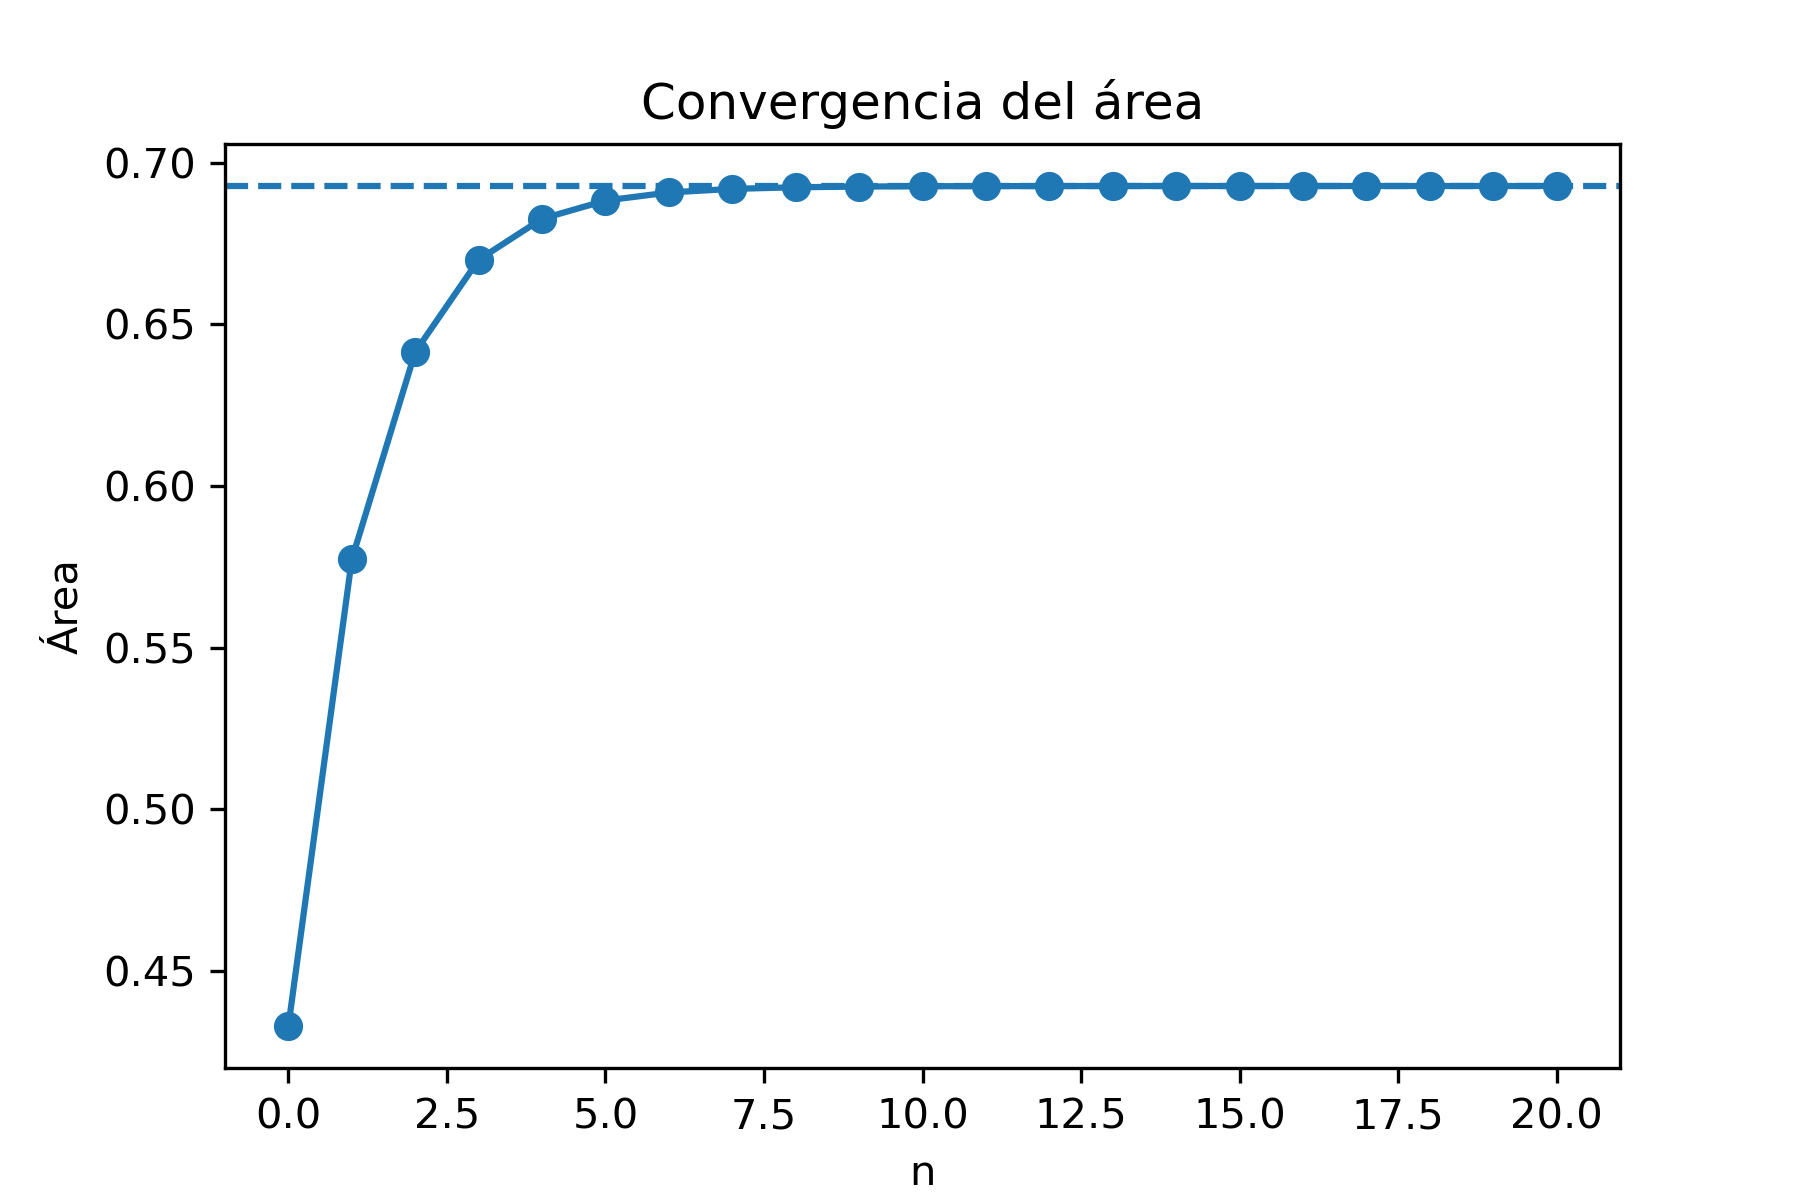
\includegraphics[width=0.6\textwidth]{imagenes/area_koch.png}
\caption{Convergencia del área del copo de Koch.}
\end{figure}

Los resultados numéricos muestran claramente esta convergencia hacia el valor teórico.

\subsubsection{Dimensión fractal}

La curva de Koch tiene una dimensión fractal no entera cuyo valor es:

\begin{equation}
D = \frac{\ln 4}{\ln 3}
\end{equation}

Para estimar numéricamente esta dimensión, se ha utilizado el método de box-counting, que consiste en cubrir la curva con cajas de tamaño $\varepsilon$ y contar el número mínimo de cajas necesarias $N(\varepsilon)$.

La dimensión se obtiene a partir de la relación 
$N(\varepsilon) \sim \varepsilon^{-D}$, lo que implica que:

\begin{equation}
D_f = \lim_{\varepsilon \to 0} \frac{\ln N(\varepsilon)}{\ln(1/\varepsilon)}
\end{equation}

Mediante un ajuste lineal en escala logarítmica se obtiene una estimación numérica de la dimensión fractal.

\begin{figure}[H]
\centering
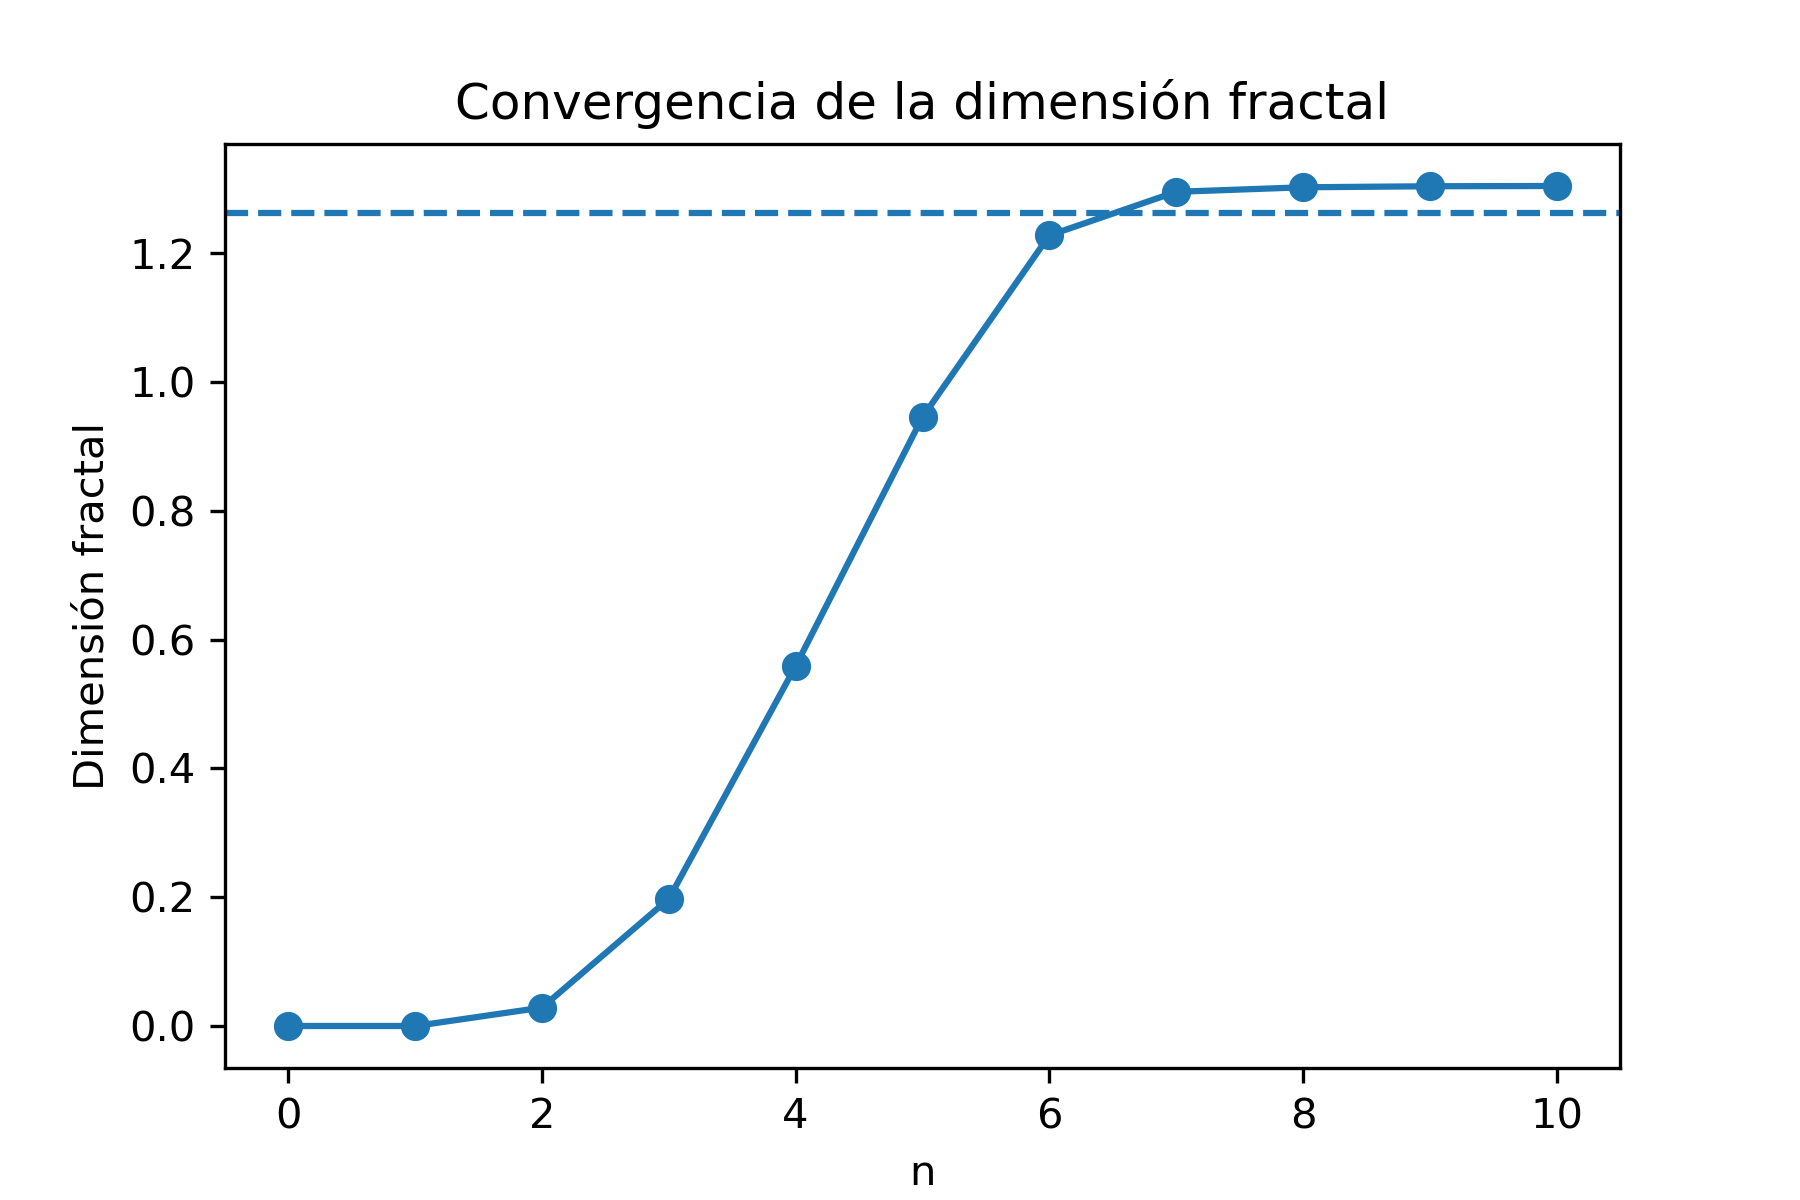
\includegraphics[width=0.6\textwidth]{imagenes/dim_fractal.png}
\caption{Convergencia de la dimensión fractal estimada mediante el método de box-counting.}
\end{figure}

Se observa que la dimensión numérica converge hacia el valor teórico al aumentar el número de iteraciones.

\section{Conclusiones}

Se ha demostrado que el paseo aleatorio reproduce el mismo comportamiento que el obtenido de las soluciones de la ecuación de difusión. También se ha estudiado la entropía de un sistema de caminantes aleatorios y se ha observado que el sistema acaba convergiendo al límite de mezcla homogénea. Finalmente, se muestra un ejemplo de sistema fractal al estudiar las curvas de Koch y sus propiedades geométricas.

\begin{thebibliography}{9}

\bibitem{giordano}
N. J. Giordano and H. Nakanishi,
\textit{Computational Physics},
2nd ed., Pearson Prentice Hall, 2006.
\label{Giordano}
\end{thebibliography}

\appendix
\section*{Anexo A: Variables}

\begin{center}
\begin{tabular}{ll}
\hline
Variable & Significado \\
\hline
$m$ & Número de caminantes \\
$N$ & Pasos temporales \\
$x,y$ & Posiciones \\
$r^2$ & Distancia cuadrática \\
$D$ & Coeficiente de difusión \\
$\rho$ & Densidad \\
$S$ & Entropía \\
$L$ & Tamaño del sistema \\
\hline
\end{tabular}
\end{center}

\end{document}